%---------------------------0-----------------------------------

\begin{frame}[c]{Geodengue}
\begin{center}
    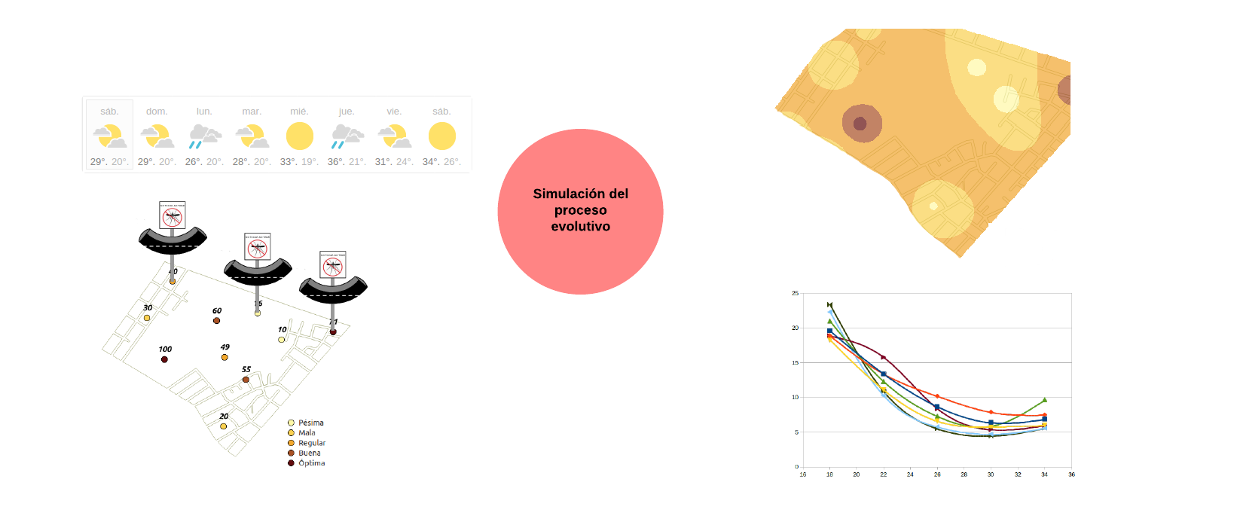
\includegraphics[width=\textwidth]{./graphics/propuesta.png}
\end{center}
\end{frame}


%----------------------------2----------------------------------
\begin{frame}[c]{Preparación de datos de entrada}
  \begin{center}
    \begin{itemize}
      \item Selección del área de estudio.
      \item Distribución geográfica de los puntos de control.
      \item Revisión de los puntos de control.
      \item Generación de la población inicial a partir de los puntos de control.
      \item Obtener datos climáticos para el periodo de simulación.
    \end{itemize}
  \end{center}
\end{frame}
%-----------------------------3---------------------------------

\begin{frame}[c]{Preparación de datos de entrada. Conteo de larvas mediante PDI.}
Utilizar procesamiento digital de imágenes para agilizar el conteo de larvas obtenidas de las larvitrampas.
    \begin{figure}
      \begin{subfigure}[b]{0.4\textwidth}
          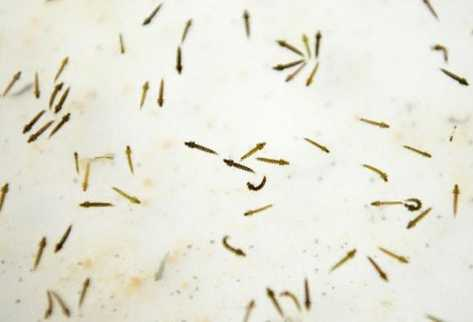
\includegraphics[width=\textwidth]{../book/capitulo-5/graphics/larvas-original.png}
          \caption{Imagen original antes de la transformación.}
      \end{subfigure}
      ~~~~
      \begin{subfigure}[b]{0.4\textwidth}
          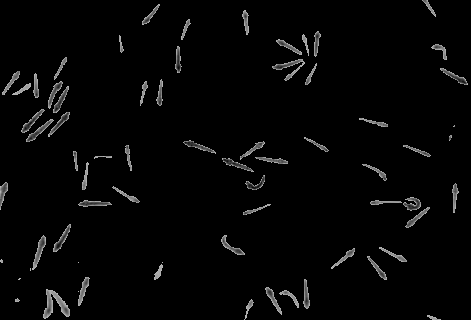
\includegraphics[width=\textwidth]{../book/capitulo-5/graphics/larvas-otsu.png}
          \caption{Imagen luego de la umbralización de Otsu.}
      \end{subfigure}
    \end{figure}
\end{frame}

%---------------------------4-----------------------------------

\begin{frame}[c]{Simulación del proceso evolutivo. Ciclo de vida del vector.}
\begin{center}
    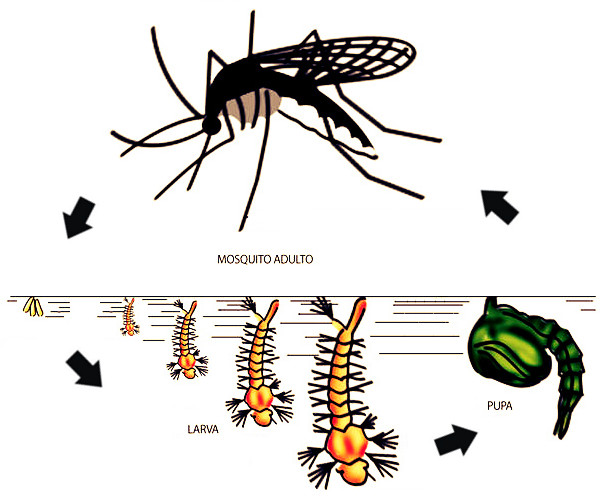
\includegraphics[width=7.8cm]{./graphics/ciclo-de-vida.jpg}
\end{center}
\end{frame}


\begin{frame}[c]{Eventos que influyen en el ciclo de vida del vector.}
  \begin{itemize}
    \item Tasas de desarrollo para la eclosión de huevos, larvas, pupas y el ciclo gonotrófico de las hembras adultas.
    \item Mortalidad de huevos, larvas, pupas y mosquitos adultos.
    \item Dispersión de adultos.
    \item Ovipostura de hembras adultas nulíperas y paridas.
  \end{itemize}
\end{frame}

\begin{frame}[c]{Simulación del proceso evolutivo. Tasas de desarrollo}
  \begin{itemize}
    \item Las tasas dependen no sólo de valores de la población, sino también de la temperatura lo que introduce una dependencia del tiempo.
    \item Se consideran 4 tasas de desarrollos : la eclosión de huevos, emergencia a pupas, emergencia a adultos y el ciclo gonotrófico.
    \item El cálculo de las tasas de desarrollo se realiza mediante el modelo no lineal de Sharpe y DeMichele.
    \item El modelo de Sharpe y DeMichele debe ajustarse con los datos biológicos disponibles.
    \item El modelo de Sharpe y DeMichele puede utilizarse para calcular tasas de desarrollo a cualquier temperatura.
  \end{itemize}
\end{frame}


\begin{frame}[c]{Simulación del proceso evolutivo. Mortalidad}

\end{frame}


\begin{frame}[c]{Simulación del proceso evolutivo. Ciclo gonotrófico y Ovipostura.}
\begin{center}
    \includegraphics[width=\textwidth]{./graphics/cliclo-gonotrofico-tiempo-2.jpg}
\end{center}
\end{frame}

\begin{frame}[c]{Simulación del proceso evolutivo. Dispersión.}
\begin{center}
  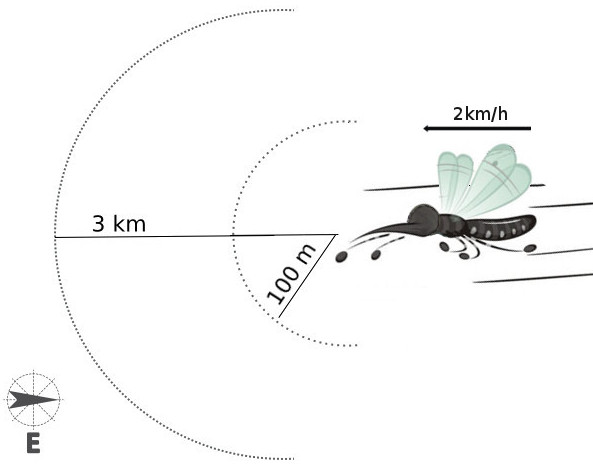
\includegraphics[width=8.5cm]{./graphics/dispersion.jpg}
\end{center}
\end{frame}


\begin{frame}[c]{Simulación del proceso evolutivo}
\begin{center}
  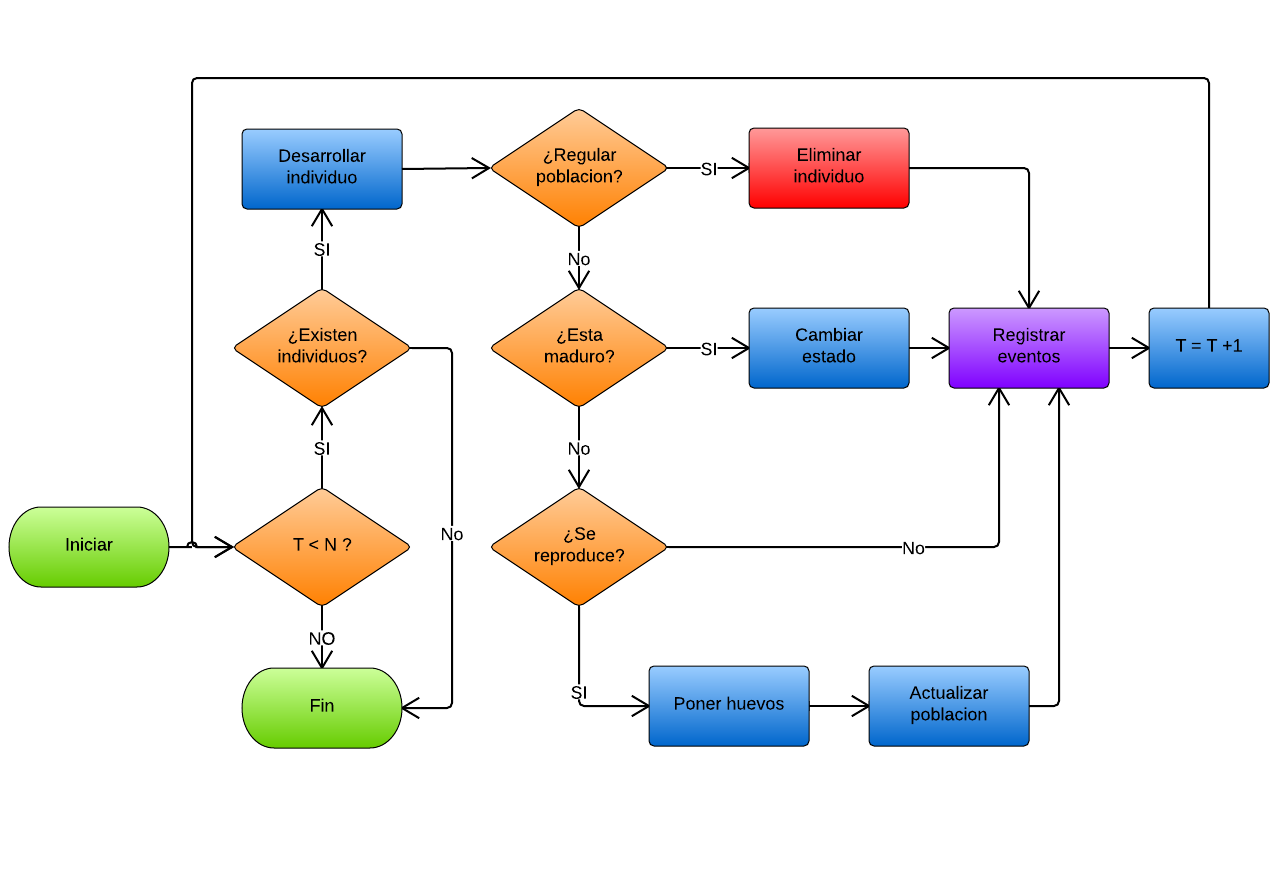
\includegraphics[height=7.5cm]{./graphics/algoritmo-propuesto.png}
\end{center}
\end{frame}

%--------------------------5------------------------------------


\begin{frame}[c]{Generación y publicación de Mapas de interpolación}
\begin{center}
    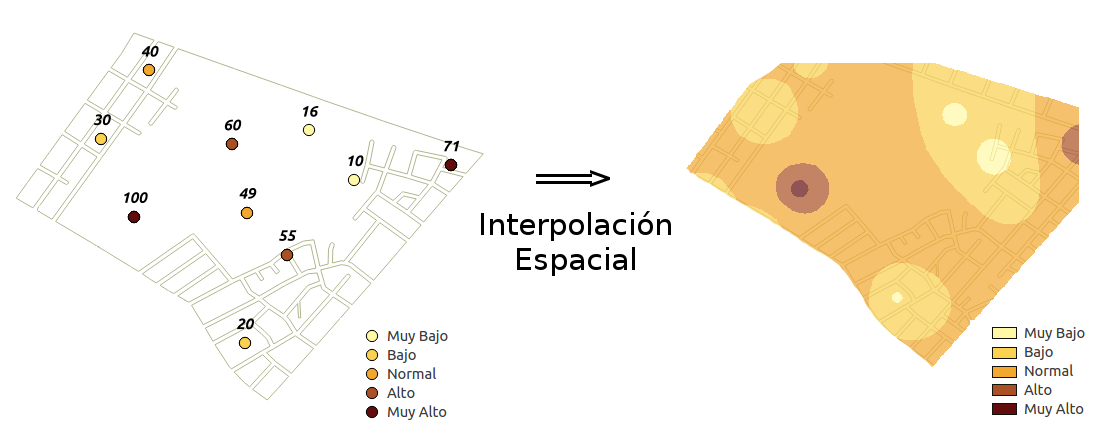
\includegraphics[width=\textwidth]{./graphics/identificacion-focos.png}
\end{center}
\end{frame}

%--------------------------6------------------------------------

\begin{frame}[t]{Análisis de los resultados}
\begin{center}
    \begin{itemize}
      \item Tasa promedio de desarrollo.
      \item Tasa promedio de mortalidad diaria.
      \item Cantidad promedio de huevos.
      \item Dispersión media.
      \item Cartografía del vector.
      \item Mapas de interpolación.
    \end{itemize}
\end{center}
\end{frame}

%--------------------------7------------------------------------

\begin{frame}[t]{Presentación de los resultados}
  \begin{itemize}
    \item Gráficos explicativos.
    \item Tablas detalladas.
    \item Mapas de interpolación como capas raster.
    \item Objetos puntuales como capas vectoriales.
  \end{itemize}
\end{frame}
